% ------------------------------------------------------------------------------
% OpenQuake-engine Users Manual
% 
% Authors: 
% 	H. Crowley 		- Executive Committee - GEM Foundation, Pavia, Italy
% 	D. Monelli 		- GEM Model Facility, Zurich, Switzerland
% 	M. Pagani 		- Executive Committee - GEM Foundation, Pavia, Italy
% 	V. Silva 		- GEM Model Facility, Pavia, Italy
%	G. Weatherhill 	- GEM Model Facility, Pavia, Italy
% 
% Document distributed under the Common Creative License 
% © GEM Foundation, Pavia, February 2013
% ------------------------------------------------------------------------------
\documentclass[12pt,a4paper,headings=small,version=last,dvips]{scrbook}
%\documentclass[12pt,a4paper,headings=small,version=first,dvips]{scrbook}
% --------------------------------------------------------------------- Packages
%%%%%%%%%%%%%%%%%%%%%%%%%%%%%%%%%%%%%%%%%
% The Legrand Orange Book
% LaTeX Template
% Version 1.4 (12/4/14)
%
% This template has been downloaded from:
% http://www.LaTeXTemplates.com
%
% Original author:
% Mathias Legrand (legrand.mathias@gmail.com)
%
% License:
% CC BY-NC-SA 3.0 (http://creativecommons.org/licenses/by-nc-sa/3.0/)
%
% Compiling this template:
% This template uses biber for its bibliography and makeindex for its index.
% When you first open the template, compile it from the command line with the 
% commands below to make sure your LaTeX distribution is configured correctly:
%
% 1) pdflatex rmtk-docs
% 1a) pdflatex -shell-escape rmtk-docs
% 2) makeindex rmtk-docs.idx -s StyleInd.ist
% 3) biber rmtk-docs
% 4  makeglossaries rmtk-docs
% 4) pdflatex rmtk-docs x 2
%
% After this, when you wish to update the bibliography/index use the appropriate
% command above and make sure to compile with pdflatex several times 
% afterwards to propagate your changes to the document.
%
% This template also uses a number of packages which may need to be
% updated to the newest versions for the template to compile. It is strongly
% recommended you update your LaTeX distribution if you have any
% compilation errors.
%
% Important note:
% Chapter heading images should have a 2:1 width:height ratio,
% e.g. 920px width and 460px height.
%
%%%%%%%%%%%%%%%%%%%%%%%%%%%%%%%%%%%%%%%%%

%----------------------------------------------------------------------------------------
%	PACKAGES AND OTHER DOCUMENT CONFIGURATIONS
%----------------------------------------------------------------------------------------

\documentclass[11pt,fleqn]{book} % Default font size and left-justified equations

\usepackage[top=3cm,bottom=3cm,left=3.2cm,right=3.2cm,headsep=10pt,a4paper]{geometry} % Page margins

\usepackage{xcolor} % Required for specifying colors by name
\definecolor{ocre}{RGB}{243,102,25} % Define the orange color used for highlighting throughout the book

% Font Settings
\usepackage{avant} % Use the Avantgarde font for headings
%\usepackage{times} % Use the Times font for headings
\usepackage{mathptmx} % Use the Adobe Times Roman as the default text font together with math symbols from the Sym­bol, Chancery and Com­puter Modern fonts

\usepackage{microtype} % Slightly tweak font spacing for aesthetics
\usepackage[utf8]{inputenc} % Required for including letters with accents
\usepackage[T1]{fontenc} % Use 8-bit encoding that has 256 glyphs

% Bibliography
\usepackage{csquotes}
\usepackage[style=alphabetic,
            sorting=nyt,
            sortcites=true,
            natbib=true,
            style=authoryear,
            maxcitenames=2,
            maxbibnames=100,
            autopunct=true,
            babel=hyphen,
            hyperref=true,
            doi=true,
            abbreviate=false,
            backref=true,
            backend=biber,
	    	uniquename=false,
	    	uniquelist=false]{biblatex}
\addbibresource{./bibliography/rmtk.bib} % BibTeX bibliography file
\defbibheading{bibempty}{}

% Figure caption settings
\usepackage[textfont=it,margin=10pt,font=small,labelfont=bf,labelsep=endash]{caption}
\usepackage{subcaption}
\usepackage{rotating}

% Table - colors from
\usepackage{verbatim}
\usepackage{color, colortbl}
\definecolor{almond}{rgb}{0.94, 0.87, 0.8}
\definecolor{ashgrey}{rgb}{0.7, 0.75, 0.71}
\definecolor{anti-flashwhite}{rgb}{0.95, 0.95, 0.96}
\definecolor{airforceblue}{rgb}{0.36, 0.54, 0.66}

% Index
\usepackage{calc} % For simpler calculation - used for spacing the index letter headings correctly
\usepackage{makeidx} % Required to make an index
% \setcounter{tocdepth}{3}    % entries down to \subsubsections in the TOC
\makeindex % Tells LaTeX to create the files required for indexing

\usepackage{todonotes}
\usepackage{geometry}
\usepackage{marginnote}

%
% Package to create a glossary - It must be uploaded after hyperref
% to produce the glossary: makeglossaries OQB
\usepackage[acronym,nonumberlist,style=altlist]{glossaries}
\glstoctrue
\makeglossaries

% package for bold symbols
\usepackage{bm}

% for better looking tables
\usepackage{ctable}
\usepackage{microtype}

% for listing Python code
\usepackage{listings}

%
%----------------------------------------------------------------------------------------
% Trees
%\usepackage[pdf]{pstricks}
%\usepackage{auto-pst-pdf}
%\usepackage{pst-tree}
%
% =============================================================== BEGIN DOCUMENT
% -------------------------------------------------- Title and table of contents
\begin{document}
% - - - - - - - - - - - - - - - - - - - - - - - - - - - - - -  Load the glossary
% OpenQuake Book Glossary 
% To cite a glossary element in a document:
%	\gls{seismicsourcedata}
%	\Gls{seismicsourcedata} - First initial is uppercase
%	\GLS{seismicsourcedata} - All initials are uppercase
%	\glspl{seismicsourcedata} - Plural
% To process the glossary:
% 	makeglossaries oqb

%
% ------- A
\newglossaryentry{areasource}{
	name = area source,
	description={A source type usually adopted to model distributed 
	seismicity. In an area source the seismicity occurrence rate 
    is assumed uniform over the source area; this produces an hazard 
    pattern with a plateau of constant hazard inside the polygon 
    delimiting the area source and values of hazard that tend to 
    decrease as we move away from the border of the source}
}
\newglossaryentry{asset}{
    name = asset,
    description={An asset is an element with a certain value, which can include buildings or population. For example, an asset can include an individual building at a given location, or a number of buildings that are grouped, co-located at a single location and classified with the same \gls{taxonomy}}.  
}
%
% ------- B
\newglossaryentry{branch}{
	name = branch,
	plural= branches,
	description={
	The simplest element in a logic tree; it belongs to a 
	\gls{branchset} where it represents one possible option among a finite 
	number of alternatives. A branch is associated with a weight 
	value \citep{scherbaum2011} if the \gls{branchset} represents the 
	epistemic uncertainty on a parameter or a model when the \gls{branchset} 
	is used to specify alternative models (e.g. district \glspl{acr:mfd})
	}
}
\newglossaryentry{branchinglevel}{
	name = branching level,
	description={It indicates the position where a \gls{branchset} or a 
	\gls{branch} is located in a logic tree structure. For example, 
	the first branching level of the 
	\gls{seismicsourcelogictree} always contains one or several 
	\glspl{initialseismicsourceinputmodel}
	}
}
\newglossaryentry{branchset}{
	name = branch set,
	description={The structure describing the epistemic uncertainty on 
	a specific parameter or model included in a logic tree structure. 
	It ensembles a number of \glspl{branch}, each one representing a 
	discrete alternative}
}
%
% ------- C
\newacronym{cpsha}{cPSHA}{Classical PSHA}
\newglossaryentry{configurationfile}{
	name =  configuration file,
	description = {
	Usually the file containing the information necessary to run a calculation
	in OpenQuake
	}
}
\newglossaryentry{charfaultsource}{
	name = characteristic fault source,
	description={
	A fault source typology where ruptures always cover the entire fault surface
	}
}
\newglossaryentry{complexfaultsource}{
	name = complex fault source,
	description={
	A source typology usually adopted to model subduction interface faults
	}
}
%
% ------- D

\newglossaryentry{deductible}{
	name = deductible,
	description = {A parameter used in the calculation of insured losses that establishes the economic value that needs to be deducted from the ground-up losses.}
}

\newglossaryentry{seismichazarddisaggregation}{
	name =  seismic hazard disaggregation,
	description = {
	A methodology to investigate the contributions to a specific
	level of hazard in terms of fundamental variables commonly used
	to characterize seismic sources and ground motion models (e.g. 
	magnitude, source-site distance, \gls{epsilon}}
}
\newglossaryentry{dip}{
	name = dip,
	description={
    The dip is the steepest angle of descent of the fault plane
    relative to a horizontal plane; it is measured in degrees [0,90] 
	}
}
\newglossaryentry{disaggregationmatrix}{
	name =  disaggregation matrix,
	description = {
	A multi-dimensional matrix used to systematically store the contributions
	to a level of hazard to be disaggregated and that is specified by the 
	user.
	See also \gls{seismichazarddisaggregation}}
}
%
% ------- E
\newacronym{acr:erf}{ERF}{Earthquake\- Rup\-ture\- Forecast}
\newacronym{acr:epsha}{ePSHA}{Event-based PSHA}
%
\newglossaryentry{earthquakeruptureforecast}{
	name = earthquake rupture forecast,
	description={
	A list of all possible ruptures generated by all the sources included 
	in a seismic source model. Each element in the list contains: the rupture 
	geometry and the rupture probability of occurrence in a given time span. 
	%
	See also the definition available on the 
	\href{http://www.opensha.org/glossary-earthquakeRuptureForecast}
	{OpenSHA website}}
}
\newglossaryentry{earthquakeruptureforecastcalculator}{
	name = earthquake rupture forecast calculator,
	description={
	Calculator producing a \gls{seismicsourcemodel} from a 
	\gls{seismicsourcelogictree} 
	}
}
%
\newglossaryentry{epsilon}{
	name = epsilon,
	description={
	normalized residual of the ground motion}
}
\newglossaryentry{exposure model}{
	name = exposure model,
	description={
	A set of \glspl{asset} grouped according to their geographical location, 
	\gls{taxonomy} and value}
}
%
% ------- F
\newglossaryentry{faulttrace}{
	name = fault trace,
	description={A curve representing the intersection between the surface 
    containing the fault surface (or its prolongation) 
	and the topographic surface.
    \begin{figure}[!ht]
    \centering
    \includegraphics[width=10cm]{./figures/hazard/single_rupture.eps}
    \end{figure}
    }
}
\newglossaryentry{fragility function}{
	name = fragility function,
	description = {the probability of exceeding a set of limit states, 
	given an intensity measure level. These functions can be discrete or
	continuous}
}
\newglossaryentry{fragility model}{
	name = fragility model,
	description = {A set of \glspl{fragility function} used to model the 
	fragility of all the \glspl{asset} in the \gls{exposure model}.}
}
\newglossaryentry{frequencymagnitudedistribution}{
	name = magnitude-frequency distribution,
	description = {See \gls{mfd}
	}
}
%
% ------- G
\newacronym{acr:gem}{GEM}{Global Earthquake Model}
\newacronym{acr:gmf}{GMF}{Ground Motion Field}
\newacronym{acr:gmpe}{GMPE}{Ground Motion Prediction Equation}
\newacronym{acr:gmlt}{GMLT}{Ground Motion Logic Tree (see 
    \gls{groundmotionlogictree}} 
\newglossaryentry{gridsource}{
	name = grid source,
	description={
	It's a source typology usually adopted to model distributed 
	seismicity. It's routinely produced by a seismicity smoothing 
	algorithm (one of the most famous algorithm is the one proposed 
	by \citet{frankel1995})}
}
\newglossaryentry{groundmotionfield}{
	name = ground-motion field,
	description={An object describing the geographic distribution around 
	a rupture of a ground motion intensity measure}
}
\newglossaryentry{groundmotionfieldcalc}{
	name = ground-motion field calculator,
	description={An \gls{acr:oqe} calculator that given a rupture computes the 
	geographic distribution of a ground motion intensity parameter. Currently
	OQ can generate ground motion fields using a \gls{acr:gmpe}}
}
\newglossaryentry{groundmotionlogictree}{
	name = ground-motion logic tree,
	description={A method used to systematically describe the epistemic 
	uncertainties related to the ground motion models used in the 
	computation of hazard using a specific \gls{pshainputmodel}}
}
\newglossaryentry{groundmotionmodel}{
	name = ground-motion model,
	description={An object that given a rupture with specific properties
	computes the expected ground motion at the given site. In simplest case 
	a ground motion model corresponds to a \gls{groundmotionpredictioneq}. 
	In case of complex PSHA input models, the produced ground motion models 
	contains a set of \glspl{acr:gmpe}, one for each tectonic region considered.
	}
}
\newglossaryentry{groundmotionparameter}{
	name = ground-motion parameter,
	description={A scalar or vector quantity describing a relevant property
	    of the shaking such as intensity (e.g. PGA or Spectral Acceleration) 
	    or duration, equivalent number of cycles 
	    \citep[see for example][]{hancock2005})
	}
}
\newglossaryentry{groundmotionpredictioneq}{
	name = ground-motion prediction equation,
	description={
		An equation that - given some fundamental parameters characterizing 
		the source, the propagation path and the site (in the simplest 
		case magnitude, distance and V$_\text{S,30}$) - computes the 
		value $GM$ of a (scalar) ground motion intensity parameter.
	}
}
\newglossaryentry{groundmotionsystem}{
	name = ground-motion system,
	description={An object containing a list of \gls{groundmotionlogictree}}
}
%
% ------- I 
\newglossaryentry{initialseismicsourceinputmodel}{
	name = initial seismic source input model,
	description={It's the ensable of information needed to fully describe 
        the seismic sources composing a seismic source input model. The 
        initial seismic source input model is included in the first 
	    branching level of a seismic source logic tree}
}

\newglossaryentry{insured losses}{
	name = insured losses,
	description = {Fraction of the ground-up losses that can be covered by the insurance industry, according to a certain policy.}
}

\newglossaryentry{investigationtime}{
	name = investigation time,
	description={The time interval considered to calculate hazard; usually 
	it corresponds to 50 years}
}
%
% ------- L
\newglossaryentry{limit}{
	name = limit,
	description = {A parameter used in the calculation of insured losses that establishes the maximum economic amount that can be covered by the insurance industry, according to a certain insurance policy.}
}
\newglossaryentry{logictree}{
	name = logic tree,
	description={Data structure used to systematically describe uncertainties
	on parameters and models used in a PSHA study}
}
\newglossaryentry{logictreeprocessor}{
	name = logic tree processor,
	description={An OQ calculator that takes the PSHA Input Model and creates 
	many realisations of a \gls{seismicsourcemodel} and of a 
	\gls{groundmotionmodel}}
} 
\newacronym{acr:ltmcs}{LTMCS}{Logic Tree Monte Carlo Sampler}
%
%
\newglossaryentry{msr}{
    name = magnitude-scaling relationship,
    description={
        An empirical relationship linking the magnitude with a parameter
        describing the size of the corresponding rupture (e.g. the area 
        of the rupture or the rupture length)
    }
}
\newacronym{acr:mfd}{MFD}{Magnitude-Frequency Distribution}
\newglossaryentry{mfd}{
    name = magnitude-frequency distribution,
    description={
   	    A distribution describing the frequency of earthquakes with 
        a specific magnitude. It can be continuous or discrete. 
        One frequency-magnitude distribution frequently adopted in 
        \gls{acr:psha} is the double truncated Gutenberg-Richter 
        distribution
    }
}
%
% ------- O
\newacronym{acr:hazlib}{oq-hazardlib}{OpenQuake hazard library}
\newglossaryentry{opensha}{
	name = OpenSHA,
	description = {OpenSHA is an open-source, advanced Java-based 
	platform for conducting Seismic Hazard Analysis - 
	(see \href{http://opensha.org}{OpenSHA website})}
}
\newacronym{acr:oqe}{oq-en\-gine}{OpenQuake-engine}
%
% ------- P
\newacronym{acr:pga}{PGA}{Peak Ground Acceleration}
\newacronym{acr:pgv}{PGV}{Peak Ground Velocity}
\newacronym[description={\glslink{psha}{Probabilistic 
    Seismic Hazard Analysis}}]{acr:psha}{PSHA}{Probabilistic Seismic 
    Hazard Analysis}
\newglossaryentry{pointsource}{
	name=point source, 
	description={The elemental source typology used in OpenQuake-engine to 
	model distributed seismicity}	
}
\newglossaryentry{pshainputmodel}{
	name=PSHA input model, 
	description={An object containing the information necessary to describe 
	the seismic source and the ground motion models - plus the related 
	epistemic uncertainties}	
}
\newglossaryentry{psha}{
	name = probabilistic seismic hazard analysis, 
	description={A methodology to compute seismic hazard by taking into 
	account the potential contributions coming from all the sources 
	of engineering importance for a specified site}	
}
%
% ------- R
\newacronym{acr:rrup}{$\text{r}_{\text{rup}}$}{closest distance between 
	the site and rupture}
\newglossaryentry{rupture}{
	name=earthquake rupture, 
	description={A 3D surface - representing a portion or the entire 
    fault surface - over which a slip event (i.e. an earthquake) 
    occurs.
	}	
}
\newglossaryentry{ruptureaspectratio}{
	name=rupture aspect ratio, 
	description={It's the ratio between the lenght and the width of an
		earthquake rupture
	}	
}
\newglossaryentry{rake}{
	name=rake, 
	description={The 
	}	
}
%
% ------- S
\newacronym{acr:ssha}{SSHA}{Scenario Based Seismic Hazard Analysis}
\newglossaryentry{scenariohazard}{
	name = scenario based seismic hazard analysis,
	plural= scenario based seismic hazard analyses,
	description = {An analyis of seismic hazard based on the selection of
        one or a few ruptures and the computation of the expected ground 
        motion at a set of sites using a \gls{gmpe} accounting ground motion
        variability.
	}
}
\newglossaryentry{seismicityhistory}{
	name = seismicity history,
	plural= seismicity histories,
	description = {An object containing a set ruptures  
	representative of the possible seismicity generated by the 
	sources in a \gls{seismicsourcemodel} during the investigation 
	time $t$
	}
}
\newglossaryentry{seismicityrate}{
	name = seismicity rate,
	description = {Number of events per unit of time (if not better 
	specified, the definition of a seismicity rate generally presumes 
	a time independent 
	}
}
\newglossaryentry{seismicsourcedata}{
	name = seismic source data,
	description={An object containing the information necessary 
	to completely describe a \gls{acr:psha} seismic source i.e. seismic 
	source type, position, geometry and seismicity occurrence 
	model}
}
\newglossaryentry{seismicsourcelogictree}{
	name = seismic source logic tree,
	description={Logic tree structure defined to describe in 
	structured and systematic way the epistemic uncertainties 
	characterizing the seismic source model. The first 
	branching level in the logic tree by definition contains one or
	several alternative \gls{initialseismicsourceinputmodel}}
}
\newacronym{acr:ssim}{SSIM}{Seismic Source Input Model}
\newglossaryentry{seismicsourceinputmodel}{
	name = seismic source input model,
	description={An object containing a list of \gls{seismicsourcedata}.
    In the OpenQuake-engine a seismic source model doesn't contain 
    epistemic uncertainty}
}
\newglossaryentry{seismicsource}{
	name = seismic source,
    description={An object that can generate}
}
\newacronym{acr:ssm}{SSM}{Seismic Source Model}
\newglossaryentry{seismicsourcemodel}{
	name = seismic source model,
	description={An object containing a list of \glspl{seismicsource}
    objects}
}
\newacronym{acr:scec}{SCEC}{Southern California Earthquake Center}
\newglossaryentry{seismicsourcesystem}{
	name = seismic source system,
	description={An object containing a list of 
        \glspl{initialseismicsourceinputmodel}
	and the \gls{seismicsourcelogictree}}
}
\newglossaryentry{simplefaultsource}{
	name = simple fault source,
	description={
	A source typology usually adopted to model shallow structures with an
	uncomplicated geometry
	}
}
\newacronym{acr:ses}{SES}{Stochastic Event Set}
\newglossaryentry{stochasticeventset}{
	name = stochastic event set,
	description={An object containing one or many \glspl{seismicityhistory} 
	}
}
\newglossaryentry{strike}{
	name = strike,
	description={
	The strike direction correspond to the angle between the north and
	the direction you take so that when you walk along the \gls{faulttrace}
	the fault dips on your right. 
	}
}
\newacronym{acr:sa}{S$_a$}{Spectral Acceleration}
%
% ------- T
\newglossaryentry{taxonomy}{
	name = taxonomy,
	description = {Scheme used to classify the \glspl{asset}. For buildings,
	a classification scheme has been proposed by \gls{acr:gem} which considers
	a number of attributes including lateral load resisting system and its 
	material, height, year of construction. The taxonomy is currently used to 
	link the \glspl{asset} in the \gls{exposure model} to the relevant 
	\gls{vulnerability function} or \gls{fragility function}}
}
\newglossaryentry{tectonicregion}{
	name = tectonic region,
	description = {A area on the topographic surface that can be considered 
	homogeneous in terms of tectonic properties such as the prevalent 
	seismogenic properties and/or the seismic wave propagation properties
	}
}
\newglossaryentry{temporaloccurrencemodel}{
	name = temporal occurrence model,
	description = {Usually a probabilistic model giving the probability of
	occurrence of an event in a specified \gls{investigationtime}
	}
}
%
% ------- U
\newacronym{acr:usgs}{USGS}{United States Geological Survey}
%
% ------- V 
\newglossaryentry{vulnerability function}{
	name = vulnerability function,
	description = {A function that describes the probability distribution
	of loss ratio, conditioned on an intensity measure level. Currently only 
	discrete vulnerability functions are supported}
}


\newglossaryentry{vulnerability model}{
	name = vulnerability mod\-el,
	description = {A set of \glspl{vulnerability function} used to model the 
	physical vulnerability of all the \glspl{asset} in the \gls{exposure model}.}
}
\newglossaryentry{acr:vs30}{
	name = V$_{S,30}$,
	description = {Average shear wave velocity of the materials in the uppermost 30m of the soil column}
}
	

% - - - - - - - - - - - - - - - - - - - - - - - - - - - - - - - - - - - -  Cover
% - - - - - - - - - - - - - - - - - - - - - - - - - - - - - - - - - - - -  Cover
%  - - - - - - - - - - - - - - - - - - - - - - - - - - - - - - - - - Second page
\restoregeometry
\cleardoublepage
%
% - - - - - - - - - - - - - - - - - - - - - - -  This is the internal title page
\setcounter{page}{1}
\begin{titlepage}
	\titlehead{\emph{``OpenQuake: Calculate, share, explore''}}
	\title{ \textcolor{blue01}{\textsf{\bfseries\Huge OpenQuake Engine User Instruction Manual}}  }
	\date{}
\end{titlepage}
\pagestyle{scrheadings}
\maketitle
%
%\input{./Part_Introduction/acknowledgements.tex}
\cleardoublepage
%
\tableofcontents
% ==============================================================================
% ------------------------------------------------------------------------- Part
\part{Risk Modeller's Toolkit}
% ------------------------------------------------------------------------------
\chapter{Nonlinear Static Method with dispersion information}
	

\section{How to use the NSP}
\label{sec:NSP}


\section{C$_R$-based procedure}
\label{sec:CR}
\subsection{Theoretical background}
The aim of this procedure, proposed by Vamvatsikos (2014), is the estimation of the median spectral acceleration value $\hat{S}_{a,ds}$, that brings the structure to the attainment of a set of damage states ds, and the corresponding dispersion beta $\beta_{S_a}$, the parameters needed for the mathematical representation of fragility in equation \ref{eq:fragility-definition}. The aim is achieved making use of the work by Ruiz-Garcia and Miranda (2007), where the inelastic displacement demand is related to the elastic displacement with a simple relationship, and it can thus be easily estimated through a response spectrum analysis and a capacity curve.

The C$_R$-based procedure presented herein is applicable to bilinear elasto-plastic capacity curve only, and it is suitable for single building fragility curve estimation, as described in section \ref{subsubsec:single-building}. However the fragility curves derived for single buildings can be combined in a unique fragility curve, which considers the inter-building uncertainty, as described in section \ref{subsubsec:multiple-building}.

\subsubsection{Single Building Fragility and Vulnerability function}
\label{subsubsec:single-building}
This procedure provides a simple relationship between median damage state threshold, expressed in terms of top displacement $\delta_{roof}$, at each damage state threshold ds, and the corresponding median elastic Spectral displacement value $\hat{S}_{d,ds}(T_1)$.

\begin{equation}
\hat{\delta}_{roof, ds} = C_R S_{d, ds}(T_1) \Gamma_1 \Phi_1
\end{equation}

where $\Gamma_1 \Phi_1$ is the first mode participation factor estimated for the first-mode shape normalised by the roof displacement, and C$_R$ is the inelastic displacement ratio (inelastic over elastic spectral displacement), computed by Ruiz-Garcia and Miranda (2007) for nonlinear SDoF systems having hysteretic behaviour representative of the analysed structure, which is a function of the first-mode period of vibration and the relative lateral strength of the system R. Therefore the median Spectral acceleration at the fundamental period of vibration $\hat{S}_{a,ds}(T_1)$ turns out to be expressed as a function of the roof displacement according to the following equation:

\begin{equation}
\hat{S}_{a,ds}(T_1) = \frac{4 \pi^2}{\hat{C}_R T^2 \Gamma_1 \Phi_1} \hat{\delta}_{roof, ds}
\label{eq:Sa_RGM}
\end{equation}

Default values of $\hat{C}_R$ parameter estimates are provided by Ruiz-Garcia and Miranda (2007), as result of nonlinear regression analysis of three different measures of central tendency computed from 240 ground motions:

\begin{equation}
\hat{C}_R = 1 + \frac{R - 1}{79.12 T_1 ^{1.98}}
\label{eq:Cr_RGM}
\end{equation}

and values for R are given as:

\begin{equation}
R_{ds} = max(0.425(1 - c + \sqrt{c^2 + 2c(2 \mu_{ds} - 1) + 1}),1)
\label{eq:R_RGM}
\end{equation}

where c = 79.12 T$^{1.98}$, and $\mu_{ds}$ is the ductility at the damage state threshold of interest.

For what concerns the dispersion of $\hat{S}_{a,ds}$, $\beta_{S_a}$, the following relationship between S and the median EDP damage threshold $\hat{\theta}$ (Cornell, 2002) is used:

\begin{equation}
\hat{\theta}(S_a) = a S_a^b
\end{equation}

so that $\beta_{S_a}$ can be easily derived from the dispersion of $\theta$ due to record-to-record variability, $\beta_{\theta d}$, as in the following:

\begin{equation}
\beta_{S_a} = \frac{1}{b} \beta_{\theta d}
\label{eq:betaSa_RGM}
\end{equation}

The dispersion of $\theta$ due to record-to-record variability, $\beta_{\theta d}$ can be easily combined with the dispersion of $\theta$ due to uncertainty in the damage state threshold $\beta_{\theta c}$ as shown in the following equation:

\begin{equation}
\beta_{S_a} = \frac{1}{b} \sqrt{\beta_{\theta d}^2 + \beta_{\theta c}^2}
\label{eq:betaSc_RGM}
\end{equation}

The dispersion of $\theta$ can be obtained assuming that $d_{roof}$ and $\theta$ are proportional, and they thus share the same dispersion. Moreover the dispersion of $d_{roof}$ is the same as the dispersion of C$_R$, since they are also proportional. Finally $\beta_{\theta d}$ can be computed with the following equation, which represents Ruiz-Garcia and Miranda's (2007) estimate of C$_R$ dispersion:

\begin{equation}
\sigma_{\ln(C_R)} = \sigma_{\ln(d_{roof})} = \beta_{\theta d} =  1.975 [\frac{1}{5.876} + \frac{1}{11.749 (T + 0.1)}] [1- \exp(-0.739 (R - 1))]
\label{eq:beta_eq_RGM}
\end{equation}

To derive a discrete vulnerability function at certain intensity measure levels, the input damage-to-loss factors are applied to the probability of occurance of each damage state, extracted from the probability of exceedance of each damage state described by the fragility function. A value of loss ratio is thus defined for the vector of selected intensity measure levels.

\subsubsection{Multiple-Building Fragility and Vulnerability function}
\label{subsubsec:multiple-buildings}
If multiple buildings have been input to derive fragility function for a class of buildings all $\hat{S}_{a, blg}$ and $\beta_{S_a, blg}$ are combined in a single lognormal curve. A minimum of 5 buildings should be considered to obtain reliable results for the class. 
A new issue arises when multiple buildings are considered: the S$_a$ at the fundamental period of each building should be converted to a common intensity measure, to be able to combine the different fragility functions. A common intensity measure is selected to be S$_a$ at the period T$_{av}$, which is a weighted average of the individual buildings fundamental period T$_1$. Then each individual fragility needs to be expressed in terms of the common S$_a$(T$_{av}$), using a spectrum. FEMA P-695 far field set of 22 accelerograms was used to derive a mean uniform hazard spectrum, and the ratio between the S$_a$ at different periods is used to scale the fragility functions. It can be noted that the actual values of the spectrum are not important, but just the spectral shape. 
Median $\hat{S}_a$ is converted to the mean $\mu_{ln(S_a)}$ of the corresponding normal distribution ($\mu_{ln(S_a)} = ln(\hat{S}_a)$) and, simply scaled to the common intensity measure as follows:

\begin{equation}
\mu_{ln(S_a), blg} = \mu_{ln(S_a), blg} S(T_{av})/ S(T_{1, blg})
\end{equation}
\begin{equation}
\beta_{S_a, blg} = \beta_{S_a, blg} S(T_{av})/ S(T_{1, blg})
\label{eq:Sa(Tav)}
\end{equation}

Finally the parameters of the single lognormal curve for the class of buildings, mean and dispersion, can be computed as the weighted mean of the single means and the weighted SRSS of the inter-building and intra-building standard deviation, the standard deviation of the single means and the single dispersions respectively, as shown in the following equations:

\begin{equation}
\mu_{ln(S_a), tot} = \sum_{i=0}^{n.blg} w_{blg-i} \mu_{ln(S_a), blg-i}
\label{eq:combination-lognormals-mu}
\end{equation}
\begin{equation}
\beta_{S_a, tot} = \sqrt{ \sum_{i=0}^{n.blg} w_{blg-i} ((\mu_{ln(S_a), blg-i}-\mu_{ln(S_a), tot})^2+ \beta_{S_a, blg-i}^2})
\label{eq:combination-lognormals-sigma}
\end{equation}

The mean $\mu_{ln(S_a)}$ and total dispersion $\beta_{S_a}$ of the fragility function of the class are converted to logarithmic mean $\mu_{S_a}$ and logarithmic covariance $cov_{S_a}$ (standard deviation $\sigma_{S_a}$ over $\mu_{S_a}$), according to the following equations:

\begin{equation}
\hat{S}_a = e^{\mu_{ln(S_a)}}
\end{equation}
\begin{equation}
\mu_{S_a} = \hat{S}_a e^{\frac{\beta_{S_a}^2}{2}}
\label{eq:median-to-mean}
\end{equation}
\begin{equation}
\sigma_{S_a} = \sqrt[2]{(\beta_{S_a}^2-1) e^{2\ln{ \hat{S}_a}+\beta_{S_a}^2}}
\label{eq:dispersion-to-standard}
\end{equation}
\begin{equation}
cov_{S_a} = \frac{\sigma_{S_a}}{\mu_{S_a} }
\end{equation}

A single vulnerability function can be also obtained, from the single building vulnerability functions. The input damage-to-loss function is applied to the fragility function derived for each building. For the selected intensity measure levels a value of loss ratio $LR_{blg}$ is thus defined for each building. A discrete vulnerability function for the entire class of buildings is represented at each iml by a mean LR, $\mu_{LR,tot}$, equal tot the weighted $LR_{blg}$, and a standard deviation, $\sigma_{LR, tot}$, equal to the weighted standard deviation of all the computed $LR_{blg}$. The $\sigma_{LR, tot}$ of the fragility function of the class is converted to covariance $cov_{LR}$ (standard deviation $\sigma_{LR, tot}$ over $\mu_{LR, tot}$).

\subsection{Inputs}
\label{subsec:InputCr}
The inputs must be formatted as comma-separated value files (.csv), and saved in the folder \textit{input}, contained in the NSP directory. If any other environment different from Windows is used make sure that the "comma separated values Windows" is selected as saving option when creating the input files. 

If multiple buildings want to be analysed to consider the inter-building uncertainty the parameters relative to each building should be added as additional lines in the input tables, as shown in the examples below, otherwise a single line must be input.

If the user has already at disposal an idealised elasto-plastic pushover curve for each building, that is to say that the variable \textit{in\_type} has been set to 0, the following data need to be provided in the corresponding csv files:

\begin{enumerate}
\item First period of vibration T$_1$, corresponding modal participation factor $\Gamma_1$, normalised with respect to the roof displacement, and weight for the combination of different buildings, input in \textit{building\_parameters.csv}, as in the example below:
	\begin{table}[H]
	\centering
	\begin{tabular}{|c|c|c|c|} \hline
	\textbf{n.building} & \textbf{T$_1$} & \textbf{$\Gamma_1$} & \textbf{weights}\\ \hline
	1 & 0.32 & 1.23 & 0.2\\ \hline
	2 & 0.40 & 1.25 & 0.3\\ \hline
	... & ... & ... & ... \\ \hline
	\end{tabular}
	\end{table}
	
\item Roof displacement at each limit state LS and corresponding dispersion $\beta_{\theta c}$ input in \textit{displacement\_profile.csv}, as shown in the example below. If dispersion is unknown, $\beta_{\theta c}$ can be set equal to zero at each LS.
	\begin{table}[H]
	\centering
	\begin{tabular}{|c|c|c|c|} \hline
	\textbf{n.building} & \textbf{LS$_1$} &	\textbf{LS$_2$} &	\textbf{LS$_3$} \\ \hline
	1 & 0.066 & 0.169 & 0.23\\ \hline
	$\beta_{\theta d, 1}$ & 0.1 & 0.3 & 0.4\\ \hline
	2 & 0.08 & 0.172 & 0.25\\ \hline
	$\beta_{\theta d, 2}$ & 0.1 & 0.3 & 0.4\\ \hline	
	\end{tabular}
	\end{table}
	
\item Idealised pushover curve, input in \textit{idealised\_curve.csv} as shown below. The only required parameters are the yielding displacement $\delta_y$, the ultimate displacement $\delta_u$ and the yielding force F$_y$.

\begin{table}[H]
\centering
\begin{tabular}{|c|c|c|c|} \hline
\textbf{n.building} & \textbf{d$_y$} & \textbf{d$_u$} & \textbf{F$_y$} \\ \hline
1 & 0.09	& 0.3	 & 523\\ \hline
2 & 0.12	& 0.35	 & 400\\ \hline
... & ...	& ... & ...\\ \hline
\end{tabular}
\end{table}

\item Consequence model (loss ratio per each damage state) consistent with the defined set of damage states, input in \textit{consequence.csv}, as in the example below. A single consequence model can be input. This input is needed only if the variable \textit{vulnerability} has been set to 1.	
	\begin{table}[H]
	\centering
	\begin{tabular}{|c|c|c|} \hline
	\textbf{DS$_1$} & \textbf{DS$_2$} & \textbf{DS$_3$} \\ \hline
	0.2	& 0.5	 & 1\\ \hline
	\end{tabular}
	\end{table}
	
\end{enumerate}

If the idealised curve are not available, \textit{in\_type} = 0 can be selected and the displacements vs base shear at each time step results from a pushover analysis can be input instead. The following data need to be provided in the corresponding csv files:

\begin{enumerate}
\item T$_1$ and corresponding $\Gamma_1$, weight for the combination of different buildings, number of storeys and height of each storey, input in \textit{building\_parameters.csv}, as in the example below:
	\begin{table}[H]
	\centering
	\begin{tabular}{|c|c|c|c|c|c|c|c|c|} \hline
	\textbf{n.building} & \textbf{T$_1$} & \textbf{$\Gamma_1$} & \textbf{weights} & \textbf{n.Storey} & \textbf{H$_1$} & \textbf{H$_2$} & ... & \textbf{H$_n$} \\ \hline
	1 & 0.32 & 1.23 & 0.2 & 4 & 3 & 3 & ... & 3 \\ \hline
	2 & 0.40 & 1.25 & 0.3 & 4 & 4 & 2.7 & ... & 2.7 \\ \hline
	... & ... & ... & ... & ... & ... & ... & ... & ... \\ \hline
	\end{tabular}
	\end{table}
	
\item Displacements at each storey, at each incremental step of the pushover analysis, input in \textit{displacements\_pushover.csv}, as in the example below: 
	\begin{table}[H]
	\centering
	\begin{tabular}{|c|c|c|c|c|c|c|} \hline
	\textbf{n.building} & \textbf{n.Storey} & \textbf{Step1} & \textbf{Step 2} & \textbf{Storey 3} & ... & \textbf{Step n}\\ \hline
	1 &	1 & 0.0001 &	0.0005 &	0.001 & ... & 0.01\\ \hline
	   &	2 & 0.0003 &	0.0010 &	0.002 & ... & 0.02\\ \hline
	   &	3 & 0.0004 &	0.0016 &	0.003 & ... & 0.03\\ \hline
	   &	4 & 0.0006 &	0.0021 &	0.004 & ... & 0.04\\ \hline
	2 &	1 & 0.0001 &	0.0005 &	0.001 & ... & 0.01\\ \hline
	   &	2 & 0.0005 &	0.0012 &	0.002 & ... & 0.03\\ \hline
	   &	... & ... &	... &	... & ... & ...\\ \hline
	\end{tabular}
	\end{table}
	
\item Base shear at each incremental step of the pushover analysis input in \textit{reactions\_pushover.csv}, as in the example below:
	\begin{table}[H]
	\centering
	\begin{tabular}{|c|c|c|c|c|c|} \hline
	\textbf{n.building} &	\textbf{Step1} & \textbf{Step 2} & \textbf{Storey 3} & ... & \textbf{Step n} \\ \hline
	1 & 0.35 & 0.69 & 1.04 & ... & 29.12\\ \hline
	2 & 0.45 & 0.78 & 2.05 & ... & 40.00\\ \hline
	... & ... & ... & ... & ... & ...\\ \hline
	\end{tabular}
	\end{table}
	
\item Drift limit state and corresponding dispersion $\beta_{\theta c}$ input in \textit{limits.csv}. If dispersion is unknown, $\beta_{\theta c}$ can be set equal to zero at each limit state.
	\begin{table}[H]
	\centering
	\begin{tabular}{|c|c|c|c|} \hline
	\textbf{n.building} & \textbf{LS$_1$} &	\textbf{LS$_2$} &	\textbf{LS$_3$} \\ \hline
	1 & 0.01 &	0.025 & 0.0337\\ \hline
	$\beta_{\theta d, 1}$ &	0.1 & 0.2 & 0.25\\ \hline
	2 & 0.014 &	0.030 & 0.0430\\ \hline
	$\beta_{\theta d, 2}$ &	0.1 & 0.2 & 0.25\\ \hline
	\end{tabular}
	\end{table}

\item Consequence model (loss ratio per each damage state) consistent with the defined set of damage states, input in \textit{consequence.csv}, as in the example below. A single consequence model can be input. This input is needed only if the variable \textit{vulnerability} has been set to 1.
	\begin{table}[H]
	\centering
	\begin{tabular}{|c|c|c|} \hline
	\textbf{DS$_1$} & \textbf{DS$_2$} & \textbf{DS$_3$} \\ \hline
	0.2	& 0.5	 & 1\\ \hline
	\end{tabular}
	\end{table}
	
\end{enumerate}

\subsection{Calculation Steps}
The overall workflow of C$_R$-based procedure is summarised in this section. The option \textit{an\_type} must be set equal to 0 and the option \textit{in\_type} according to the input at disposal. The corresponding inputs should follow the requirements described in section \ref{subsec:InputCr}. At this point the code proceeds with the following steps:

\begin{enumerate}
\item
\begin{enumerate}
\item If \textit{in\_type} = 0 roof displacement at limit states and idealised pushover are extracted from \textit{displacement\_profile.csv} and \textit{idealised\_curve.csv} respectively.
\item If \textit{in\_type} = 1 results from pushover analysis are extracted from \textit{displacements\_pushover.csv} and \textit{reactions\_pushover.csv}, and drift limit states from \textit{limits.csv}. The idealised 	pushover curve is then derived in the \textit{idealisation} function, where the idealisation process is conducted according to FEMA-440. The elastic stiffness is defined as the 	tangent stiffness passing through the point of the pushover curve where 60\% of the maximum base shear is reached, and the perfectly plastic branch is set at an height equal to 	the maximum base shear. The yielding point is found as the interception between the elastic and the plastic branch.
\end{enumerate}

\item The csv input files are parsed with the function \textit{read\_data} according to the defined options. The parameters essential to the analysis are return together with a graphical visualisation of the inputs if the variable \textit{plotflag}[0] is equal to 1.

\item The parameters extracted are used in the \textit{simplified\_bilinear} function, within the \textit{fragility\_process} function, to derive ductility levels $\mu_{ds}$, median spectral acceleration $\hat{S}_{a,ds}$ and the total dispersion $\beta_{S_a}$ at each limit state through the following steps:
\begin{itemize}
\item The idealised MDoF system is transformed into an equivalent SDoF system, using $\Gamma_1$.
\item Ductility levels $\mu_{ds}$ corresponding to each damage threshold, are defined.
\item R and C$_R$ are computed, using eq. \ref{eq:R_RGM} and \ref{eq:Cr_RGM} respectively.
\item $\hat{S}_{a,ds}$ and the corresponding dispersion  $\beta_{\theta d}$ are computed using eq. \ref{eq:Sa_RGM} and \ref{eq:betaSa_RGM} respectively.
\item $\beta_{\theta d}$ is combined with dispersion due to uncertainty in the model $\beta_{\theta c}$, if different from zero, to get the total dispersion $\beta_{S_a}$, using eq. \ref{eq:betaSc_RGM}.
\item $\hat{S}_a(T_1)$ is converted to mean $\mu_{ln(S_a)}(T_1)$ and then to the intensity measure in common with the rest of the buildings, $\mu_{ln(S_a(T_{av}))}$, according to eq. \ref{eq:Sa(Tav)}
\end{itemize}

\item Step 3. is repeated for the number of input buildings.

\item
\begin{enumerate}
\item If vulnerability = 0: All $\mu_{ln(S_a), blg}$ and $\beta_{S_a, blg}$ are combined in a single lognormal curve, whose parameters are evaluated according to equations \ref{eq:combination-lognormals-mu} and \ref{eq:combination-lognormals-sigma}. Mean $\mu_{ln(S_{a})}$ and total dispersion $\beta_{S_a}$ are then converted to logarithmic mean $\mu_{S_a}$ and logarithmic covariance $cov_{S_a}$, according to equations \ref{eq:median-to-mean} and \ref{eq:dispersion-to-standard} respectively. Fragility curves for the class of buildings are displayed if the variable \textit{plotflag}[2] = 1, and logarithmic $\mu_{S_a}$ and $cov_{S_a}$ are exported in the \textit{outputs} folder.

\item If vulnerability =1: Vulnerability curves are derived for each fragility function derived at step 4. For the intensity measure levels defined in the variable \textit{iml} a value of loss ratio is thus defined for each building. They are finally combined in a single mean and its standard deviation, equal to the weighted mean and the weighted standard deviation of the loss ratios, as described in section \ref{subsec:InputCr}. Vulnerability curve for the class of buildings is displayed if the variable \textit{plotflag}[3] = 1. The $\sigma_{LR, tot}$ of the fragility function of the class is converted to covariance $cov_{LR}$ and $\mu_{LR}$ and $cov_{LR}$ at each iml are exported in the \textit{outputs} folder.
\end{enumerate}
\end{enumerate}

\section{Spo2ida-based procedure}
\label{sec:spo2ida}
\subsection{Theoretical background}
The aim of this procedure is the estimation of the median spectral acceleration value $\hat{S}_{a,ds}$, that brings the structure to the attainment of a set of damage states ds, and the corresponding dispersion beta $\beta_{S_a}$, the parameters needed for the mathematical representation of fragility in equation \ref{eq:fragility-definition}. The aim is achieved making use of the tool spo2ida (Vamvatsikos and Cornell, 2006), where static pushover curves are converted into 16\%, 50\% and 84\% IDA curves, using empirical relationships from a large database of incremental dynamic analysis results, as shown in Figure~\ref{fig:spo2ida}.

\begin{figure}[H]
\centering
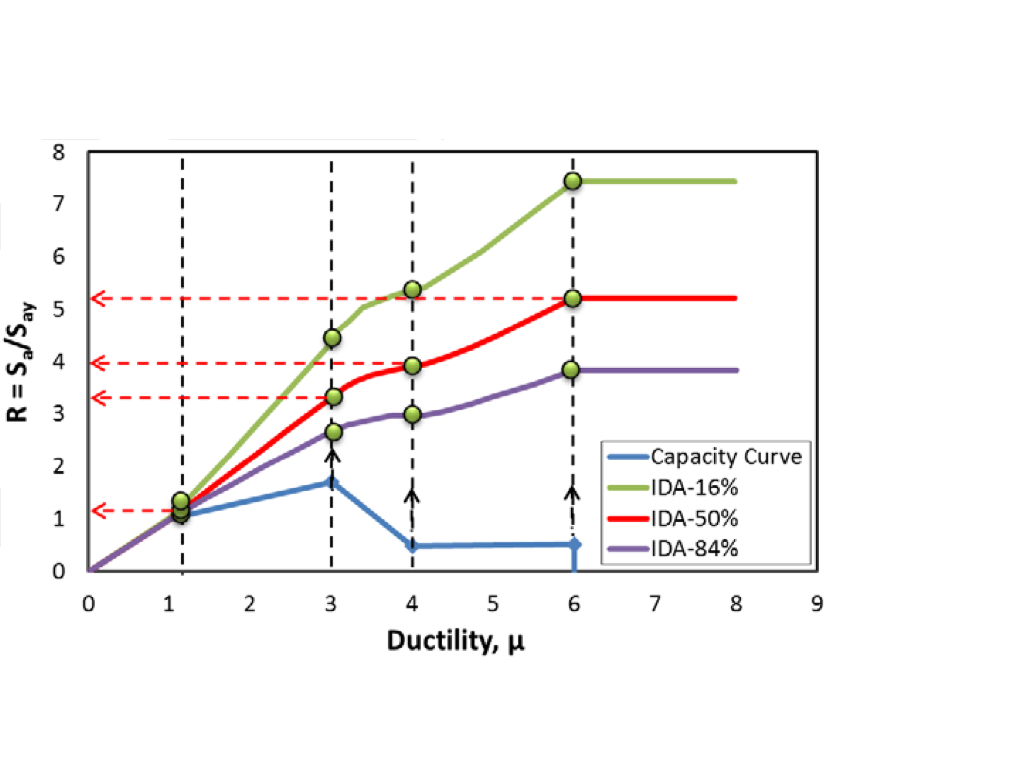
\includegraphics[width=12cm,height=8cm]{./figures/spo2ida.jpg}
\caption{spo2ida tool: IDA curves derived from Pushover curve.}
\label{fig:spo2ida}
\end{figure}

The spo2ida-based procedure presented herein is applicable to any kind of multi-linear capacity curve, and it is suitable for single building fragility curve estimation, as described in section \ref{subsubsec:single-building-spo2ida}. However the fragility curves derived for single buildings can be combined in a unique fragility curve, which considers the inter-building uncertainty, as described in section \ref{subsubsec:multiple-building-spo2ida}.

\subsubsection{Single-building Fragility and Vulnerability function}
\label{subsubsec:single-building-spo2ida}
Given the idealised capacity curve the spo2ida tool uses an implicit R-$\mu$-T relation to correlate nonlinear displacement, expressed in terms of ductility $\mu$ to the corresponding medians capacity in terms of the parameters R. R is the lateral strength ratio, defined as the ratio between the spectral spectral acceleration S$_a$ and the yielding capacity of the system S$_{ay}$. 

Each branch of the capacity curve, hardening, softening and residual plateau, is converted to a corresponding branch of the three ida curves, using the R-$\mu$-T relation, which is a function of the hardening stiffness, the softening stiffness and the residual force. These parameters are derived from the idealised pushover capacity expressed in $\mu$-R terms, as well as the ductility levels at the onset of each branch. If some of the branches of the pushover curve are missing because of the seismic behaviour of the system, spo2ida can equally work with bilinear, trilinear and quadrilinear idealisations.

The result of the spo2ida routine is thus a list of ductility levels and corresponding R values at 50\%, 16\% and 84\% percentiles. The distribution of R values at each ductility level, due to the record-to-record variability, is assumed to be lognormal and it can be easily converted to the dispersion of the lognormal distribution with the following equation:

\begin{equation}
\beta_{R(\mu)} = \frac{\ln R(\mu)_{84\%} - \ln R(\mu)_{16\%}}{2}
\label{eq:betaR}
\end{equation} 

$\beta_{R(\mu)}$ represents also the record-to-record variability of S$_a$ at different ductility levels $\beta_{S_a, d}$. Median R and its dispersion at ductility levels corresponding to the damage thresholds can thus be determined, and $\hat{S}_{a,ds}$ can be easily extracted simply multiplying $R_{50\%}(\mu_{ds})$ by the yielding capacity of the system $S_{ay}$, as shown in the following equation:

\begin{equation}
\hat{S}_{a,ds} = R_{50\%}(\mu_{ds}) S_{ay}
\label{eq:SaR}
\end{equation}
\begin{equation}
S_{ay} = \frac{4 \pi^2 \delta_{roof,y}}{g \Gamma_1 T_1^1}
\end{equation}

Since $\hat{R}$ and $\hat{S}_{a}$ are proportional they share the same dispersion.

If dispersion due to uncertainty in the limit state definition $\beta_{\theta c}$ is different from zero it can not be combined directly with the record-to-record dispersion, but a Monte Carlo sampling of the limit state needs to be performed instead. Different values of ductility limit state are sampled from the  lognormal distribution with median the median value of the ductility limit state, and dispersion the input $\beta_{\theta c}$. For each of these ductilities the corresponding R$_{16\%}$-R$_{50\%}$-R$_{84\%}$ are found and converted into $\hat{S}_{a,ds}$ and $\beta_{\theta d}$ according to equation \ref{eq:SaR} and \ref{eq:betaR}. N random S$_a$ corresponding to the N sampled ductility limit states are computed, and their median and the dispersion are estimated. These parameters constitute the median $\hat{S}_{a,ds}$ and the total dispersion $\beta_{S_a}$ for the considered damage state. The procedure is repeated for each damage state.

To derive a discrete vulnerability function at certain intensity measure levels, the input damage-to-loss factors are applied to the probability of occurance of each damage state, extracted from the probability of exceedance of each damage state described by the set of fragility curves. 

If dispersion due to uncertainty in the limit state is different from zero a vulnerability function is derived for the N sets of sampled ductility limit states. It results in N loss ratios for each defined intensity measure levels. Finally a lognormal distribution of the loss ratios is assumed at each iml and the vulnerability curve is defined at each iml by the mean and the standard deviation of all the computed loss ratios.

\subsubsection{Multiple-Building Fragility and Vulnerability function}
\label{subsubsec:multiple-building-spo2ida}
If multiple buildings have been input to derive a set of fragility curves for a class of buildings all $\hat{S}_{a,blg}$ and $\beta_{S_a,blg}$ are combined in a single lognormal curve for each damage state. A minimum of 5 buildings should be considered to obtain reliable results for the class. The procedure to get $\mu_{S_a,tot}$ and $cov_{S_a,tot}$ for the class of building is the same described in section \ref{subsubsec:multiple-buildings}, but the $\hat{S}_{a,blg}$ and $\beta_{S_a,blg}$ are those derived from each sampled set of ductility limit state.

A single vulnerability curve can also be obtained, from the single building vulnerability curves. If no dispersion in the limit state is defined, the method is the same described in section \ref{subsubsec:multiple-buildings}. Otherwise a vulnerability curve is derived for each building as explained in section \ref{subsub:single-building-spo2ida}, considering the sampled set of ductility limit states, that is to say that the mean loss ratio and its standard deviation at each iml, $\mu_{LR,iml,blg}$ and $\sigma_{LR,iml,blg}$ respectively, are found for each building.
Finally the mean loss ratio and its standard deviation, $\mu_{LR,iml}$ and $\sigma_{LR,iml}$, are found for the entire class of buildings as the weighted mean of the single $\mu_{LR,iml,blg}$ and the weighted SRSS of the inter-building and intra-building standard deviation, the standard deviation of the single means $\mu_{LR,iml,blg}$ and the single dispersions $\sigma_{LR,iml,blg}$ respectively, as described in eq \ref{eq:combination-lognormals-sigma}, substituting loss ratio to spectral acceleration.

\subsection{Inputs}
\label{subsec:InputSpo2ida}
The inputs must be formatted as comma-separated value files (.csv), and saved in the folder \textit{input}, contained in the NSP directory. If any other environment different from Windows is used make sure that the "comma separated values Windows" is selected as saving option when creating the input files. 

If multiple buildings want to be analysed to consider the inter-building uncertainty the parameters relative to each building should be added as additional lines in the tables, as shown in the examples below, otherwise a single line must be input.

If the user has already at disposal an idealised multilinear pushover curve for each building, that is to say that the variable \textit{in\_type} has been set to 0, the following data need to be provided in the corresponding csv files:

\begin{enumerate}
\item First period of vibration $T_1$, corresponding modal participation factor $\Gamma_1$, normalised with respect to the roof displacement, and weight for the combination of different buildings, input in \textit{building\_parameters.csv}, as in section \ref{subsec:InputCr}, input n. 1.
	
\item Top displacement at each damage state threshold and corresponding dispersion $\beta_{\theta c}$ input in \textit{displacement\_profile.csv}, as in section \ref{subsec:InputCr}, input n. 2. 
	
\item Idealised pushover curve, input in \textit{idealised\_curve.csv} as shown below. The parameters needed to describe the idealised pushover curve are: yielding displacement d$_y$, displacement at the onset of degradation d$_s$, displacement at the onset of residual force d$_{min}$, ultimate displacement d$_u$, maximum force F$_{max}$, residual force F$_{min}$. These parameters are represented in Figure~\ref{fig:quadrilinear}.

\begin{figure}[H]
\centering
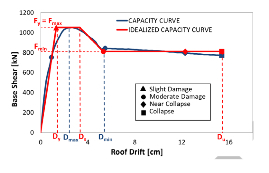
\includegraphics[width=12cm,height=8cm]{./figures/quadrilinear.jpg}
\caption{Idealisation of capacity curve using multilinear elasto-plastic form.}
\label{fig:quadrilinear}
\end{figure}

\begin{table}[H]
\centering
\begin{tabular}{|c|c|c|c|c|c|c|} \hline
\textbf{n.building} & \textbf{d$_y$} & \textbf{d$_s$} & \textbf{d$_{min}$} & \textbf{d$_u$} & \textbf{F$_{max}$} & \textbf{F$_{min}$} \\ \hline
1 & 0.09	& 0.3	& a & b & 523 & 430\\ \hline
2 & 0.12	& 0.35	 & a & b & 400 & 305\\ \hline	
\end{tabular}
\end{table}

\item Consequence model (loss ratio per each damage state) consistent with the defined set of damage states, input in \textit{consequence.csv}, as in section \ref{subsec:InputCr}, input n. 5.
	
\end{enumerate}

If these data are not available, \textit{in\_type} = 0 can be selected and the "raw" results from a pushover analysis can be input instead. The same data as in section \ref{subsec:InputCr} for \textit{in\_type} = 0 can be input.

\subsection{Calculation Steps}
The overall workflow of spo2ida-based procedure is summarised in this section. The option \textit{an\_type} must be set equal to 1 and the option \textit{in\_type} according to the input at disposal. The corresponding inputs should follow the requirements described in section \ref{subsec:InputSpo2ida}. At this point the code proceeds with the following steps:

\begin{enumerate}
\item 
\begin{enumerate}
\item If \textit{in\_type} = 0, the roof displacement at each limit state and the idealised pushover curve parameters are extracted from \textit{displacement\_profile.csv} and \textit{idealised\_curve.csv} respectively.

\item If \textit{in\_type} = 1 the results from a pushover analysis are extracted from \textit{displacements\_pushover.csv} and \textit{reactions\_pushover.csv} and drift limit states from {limits.csv}. The idealised pushover curve is then derived in the \textit{idealisation} function, where the idealisation process is conducted according to the Gem Analytical Vulnerability Guidelines.	\end{enumerate}

\item The parameters extracted are used to derive ductility levels $\mu_{ds}$, median spectral acceleration $\hat{S}_{a,ds}$ and the total dispersion $\beta_{S_a}$ at each damage threshold through the following steps:
\begin{itemize}
\item The idealised MDoF system is transformed into an equivalent SDoF system, using $\Gamma_1$, and SDoF capacity curve is  expressed in terms of $\mu$-R.

\item The variables for spo2ida tool are extracted from the capacity curve and they are used as input to get the 16\%-50\%-84\% ida curves.

\item The ductility levels $\mu_{ds}$ corresponding to each damage threshold are defined, and the corresponding R$_{16\%}$-R$_{50\%}$-R$_{84\%}$ are found in ida outputs.

\item $\hat{S}_{a,ds}$ and the corresponding dispersion $\beta_{S_{a, d}}$ are computed using eq.~\ref{eq:SaR} and eq.~\ref{eq:betaR}, respectively.

\item If dispersion due to uncertainty in the limit state $\beta_{\theta c}$ is different from zero different ductility limit states are sampled for each median ductility level $\mu_{ds}$ and corresponding values of $\hat{S}_{a,ds}$ and $\beta_{S_{a, d}}$ are computed, as described in section \ref{subsubsec:single-building-spo2ida}, but not yet combined together.

\end{itemize}

\item All $\hat{S}_{a, ds}(T_1)$ are converted to mean $\mu_{ln(S_{a, ds})}(T_1)$ and then to the intensity measure in common with the rest of the buildings, $\mu_{ln(S_{a, ds}(T_{av}))}$, according to eq. \ref{eq:Sa(Tav)}.

\item Step 2. and 3. are repeated for the number of input buildings.

\item
\begin{enumerate}

\item If vulnerability = 0: All $\hat{S}_{a,ds}$ and $\beta_{S_{a, d}}$ from all the buildings and all the sampled ductility limit states are combined in a single lognormal curve, as described in section \ref{subsub:single-building-spo2ida}. 
Mean $\mu_{ln(S_{a})}$ and total dispersion $\beta_{S_a}$ are then converted to logarithmic mean $\mu_{S_a}$ and logarithmic covariance $cov_{S_a}$, according to equations \ref{eq:median-to-mean} and \ref{eq:dispersion-to-standard} respectively.
Fragility curves for the class of buildings are displayed if the variable \textit{plotflag}[2] = 1, and logarithmic $\mu_{S_a}$ and $cov_{S_a}$ are exported in the \textit{outputs} folder.
\item If vulnerability =1:  
For the intensity measure levels defined in the variable \textit{iml} a value of loss ratio $\mu_{LR, iml, blg}$ is defined for each building and a standard deviation $\sigma_{LR, iml, blg}$, if dispersion due to uncertainty in the limit state $\beta_{\theta c}$ is different from zero. They are finally combined in a single mean and standard deviationas described in section \ref{multiple-building-spo2ida}. Vulnerability curve for the class of buildings is displayed if the variable \textit{plotflag}[3] = 1, and $\mu_{LR}$ and $cov_{LR}$ at each iml are exported in the \textit{outputs} folder.
\end{enumerate}

\end{enumerate}

\section{R-$\mu$-T procedure}
\label{sec:DF}
\subsection{Theoretical background}
The aim of this procedure is the estimation of the median spectral acceleration value $\hat{s}_c$, that brings the structure to the attainment of a set of damage states, and the corresponding dispersion beta $\beta_{sc}$, the parameters needed for the mathematical representation of fragility in equation \ref{eq:fragility-definition}. The aim is achieved making use of a R-$\mu$-T relationship, between the reduction factor R, the ductility $\mu$ and period T, which is based on the work of Dolsek and Fajfar (2004). The R-$\mu$-T-based procedure presented herein is applicable to any kind of multi-linear capacity curve, and it is suitable for single building fragility curve estimation, as described in section \ref{subsubsec:single-building-DF}. However the fragility curves derived for single buildings can be combined in a unique fragility curve, which considers the inter-building uncertainty, as described in section \ref{subsubsec:multiple-building-DF}.

\subsubsection{Single Building Fragility and Vulnerability function}
\label{subsubsec:single-building-DF}
The spectral value at each damage state threshold ds $\hat{S}_{a,ds}$ is found from the top displacement representing that ds attainment $\hat{\delta}_{roof, ds}$, as explained in C$_{R}$\_based procedure and reported the following equation:

\begin{equation}
\hat{S}_{a,ds}(T_1) = \frac{4 \pi^2}{\hat{C}_R T^2 \Gamma_1 \Phi_1} \hat{\delta}_{roof, ds}
\label{eq:basic_DF}
\end{equation}

The value of C$_R$, the ratio between the inelastic and the elastic spectral displacement, is found from equation \ref{eq:Cr_DF}.

\begin{equation}
\hat{C}_{R} = \frac{\mu_{LS}}{R_{LS}}
\label{eq:Cr_DF}
\end{equation}

where $\mu_{ds}$ and $R_{ds}$ are the ductility level and the reduction factor at each ds attainment. According to the results of an extensive parametric study using three different sets of recorded and semi-artificial ground motions Dolsek and Fajfar (2004) related the ductility demand, $\mu$ , and reduction factor, R , through the following formula:

\begin{equation}
\label{eq:mu_DF}
\mu = \frac{1}{c} (R-R_{0})+\mu_{0}
\end{equation}

In the proposed model, $\mu$ is linearly dependent on R within two reduction factor intervals. The parameter c defines the slope of the R–$\mu$ relation, and depends on the initial period of the system T, the ratio r$_{u}$, the reduction factor R and the corner periods T$_{c}$ and T$_{d}$. T$_{c}$ and T$_{d}$ are the corner periods between the constant acceleration and constant velocity part of the idealized elastic spectrum, and between the constant velocity and constant displacement part of the idealized elastic spectrum respectively.

Given the parameters of the multilinear pushover curves (R$_{\mu_{c}}$, $\mu_{c}$, r$_{u}$) and T, the median R-$\mu$ curve, similar to an IDA curve, can be construct using the aforementioned relationship.  A multilinear capacity curve and the corresponding R$_{\mu_{c}}$, $\mu_{c}$ and r$_{u}$ parameters are shown in Figure \ref{fig:quadrilinear_DF}.

\begin{figure}[H]
\centering
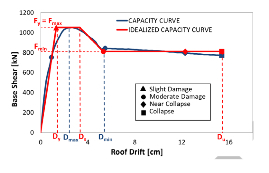
\includegraphics[width=10cm,height=5cm]{./figures/quadrilinearDF.jpg}
\caption{Multilinear capacity curve and parameters for the definition of R-$\mu$ relation.}
\label{fig:quadrilinear_DF}
\end{figure}

On the median "IDA curve" the $\mu$-R pairs corresponding to the limit states (R$_{LS}$ and $\mu_{LS}$) can be found and turned into median spectral acceleration values for that limit state $\hat{S}_c$, to be used in equation \ref{eq:basic_DF}.

Once median R$_{LS}$ and $\mu_{LS}$ are found, the 84 and 16 fractiles $\mu$ are extracted using top drift record-to-record dispersion $\sigma_{ln(\delta)}$ from equation \ref{eq:beta_eq_RGM}, by Ruiz-Garcia and Miranda (2007). The steps to derive $\mu_{16}$ and $\mu_{84}$ are the following:
 
\begin{equation}
ln(\delta)_{16} = ln(\hat{\delta})-\sigma_{ln(\delta)}
\end{equation}
\begin{equation}
ln(\delta)_{84} = ln(\hat{\delta})+\sigma_{ln(\delta)}
\end{equation}
\begin{equation}
\mu_{16} = \hat{\mu} \exp{-\sigma_{ln(\delta)}}
\end{equation}
\begin{equation}
\mu_{84} = \hat{\mu} \exp{\sigma_{ln(\delta)}}
\end{equation}

Given the linear relationship between R and $\mu$, the R$_{16}$ and R$_84$ values at $\mu_{LS}$ are just linearly interpolated, and the record-to-record dispersion of the spectral acceleration $\beta_{S_{a, d}}$ at each $\mu_{LS}$ coincides with the dispersion of R, computed from the percentiles values.

\begin{equation}
\label{eq:beta_DF}
\beta_{R(\mu)} = \frac{\ln R(\mu)_{84\%} - \ln R(\mu)_{16\%}}{2}
\end{equation} 

The dispersion of $S_{a}$ due to uncertainty in the damage state threshold $\beta_{S_{a, c}}$ can be found converting the dispersion on the damage threshold $\beta_{\theta c}$, as explaind in equation \ref{eq:betaSa_RGM} and reported in the following equation.

\begin{equation}
\label{eq:betasc_DF}
\beta_{S_{a, c}} = \frac{1}{b} \beta_{\theta c}
\end{equation}

In order to derive the b values, which represent the slope of the R-$\mu$ relation in the log-space, a further step needs to be made, because the R-$\mu$-T is suggested by the authors as conservative, since it is not based on the median but on the mean $\mu$ given R. An attempt was made to correct b reducing the median R curve by 15\%, $\hat{R}_{corrected}$, and extrapolating the corresponding $\hat{\mu}_{corrected}$.

\begin{equation}
\hat{R}_{corrected}=0.85\hat{R}
\end{equation}
\begin{equation}
\label{eq:bcorrected_DF}
b=ln(\hat{\mu}_{corrected})/ln(\hat{R}_{corrected})
\end{equation}

Finally the dispersion of $S_{a}$ due to record-to-record variability, $\beta_{S_{a, d}}$ can be easily combined with the dispersion of $S_{a}$ due to uncertainty in the damage state threshold $\beta_{S_{a, c}}$ as shown in the following equation.

\begin{equation}
\label{eq:betatotal_DF}
\beta_{S_a} = \sqrt{\beta_{S_{a, c}}^2 + \beta_{S_{a, d}}^2}
\end{equation}

\subsubsection{Multiple Building Fragility and Vulnerability function}
\label{subsubsec:multiple-building-DF}
 If multiple buildings have been input to derive fragility function for a class of buildings all $\hat{S}_{a, blg}$ and $\beta_{S_a, blg}$ are combined in a single lognormal curve as described in section \ref{subsubsec:multiple-buildings}. The same holds for vulnerability function, as described in the same section.

\subsection{Inputs}
The data the user needs provided and the their format is described in section \ref{subsec:InputSpo2ida}

\subsection{Calculation Steps}
The overall workflow of R-$\mu$-T-based procedure is summarised in this section. The option \textit{an\_type} must be set equal to 2 and the option \textit{in\_type} according to the input at disposal. The corresponding inputs should follow the requirements described in section \ref{subsec:InputSpo2ida}. At this point the code proceeds with the following steps:

\begin{enumerate}
\item 
\begin{enumerate}
\item If \textit{in\_type} = 0, the roof displacement at each limit state and the idealised pushover curve parameters are extracted from \textit{displacement\_profile.csv} and \textit{idealised\_curve.csv} respectively.

\item If \textit{in\_type} = 1 the results from a pushover analysis are extracted from \textit{displacements\_pushover.csv} and \textit{reactions\_pushover.csv} and drift limit states from {limits.csv}. The idealised pushover curve is then derived in the \textit{idealisation} function, where the idealisation process is conducted according to the Gem Analytical Vulnerability Guidelines.	\end{enumerate}

\item The csv input files are parsed with the function \textit{read\_data} according to the defined options. The parameters essential to the analysis are return together with a graphical visualisation of the inputs if the variable \textit{plotflag}[0] is equal to 1.

\item The parameters extracted are used in the \textit{DFfragility} function, within the \textit{fragility\_process} function, to derive ductility levels $\mu_{ds}$, median spectral acceleration $\hat{S}_{a,ds}$ and the total dispersion $\beta_{S_a}$ at each limit state through the following steps:
\begin{itemize}
\item The idealised MDoF system is transformed into an equivalent SDoF system, using $\Gamma_1$.
\item Ductility levels $\mu_{ds}$ corresponding to each damage threshold, are defined.
\item R and C$_R$ are computed, using eq. \ref{eq:mu_DF} and \ref{eq:Cr_DF} respectively.
\item $\hat{S}_{a,ds}$ and the corresponding dispersion  $\beta_{\S_{a, d}}$ are computed using eq. \ref{eq:basic_DF} and \ref{eq:beta_DF} respectively.
\item R$_{corrected}$ curve are found reducing by 15\% the median R curve, and the corresponding $\mu_{corrected}$ corrected are extrapolated.
\ b value is found from R and mu according to eq. \ref{eq:bcorrected_DF}.
\item Uncertainty in the model is expressed in terms of dispersion in S$_a$ $\beta_{\S_{a, c}}$ according to eq. \ref{eq:betasc_DF} and combined with $\beta_{\S_{a, d}}$ to get the total dispersion $\beta_{S_a}$, using eq. \ref{eq:betatotal_DF}.
\item $\hat{S}_a(T_1)$ is converted to mean $\mu_{ln(S_a)}(T_1)$ and then to the intensity measure in common with the rest of the buildings, $\mu_{ln(S_a(T_{av}))}$, according to eq. \ref{eq:Sa(Tav)}
\end{itemize}

\item Step 3. is repeated for the number of input buildings.

\item
\begin{enumerate}
\item If vulnerability = 0: All $\mu_{ln(S_a), blg}$ and $\beta_{S_a, blg}$ are combined in a single lognormal curve, whose parameters are evaluated according to equations \ref{eq:combination-lognormals-mu} and \ref{eq:combination-lognormals-sigma}. Mean $\mu_{ln(S_{a})}$ and total dispersion $\beta_{S_a}$ are then converted to logarithmic mean $\mu_{S_a}$ and logarithmic covariance $cov_{S_a}$, according to equations \ref{eq:median-to-mean} and \ref{eq:dispersion-to-standard} respectively. Fragility curves for the class of buildings are displayed if the variable \textit{plotflag}[2] = 1, and logarithmic $\mu_{S_a}$ and $cov_{S_a}$ are exported in the \textit{outputs} folder.

\item If vulnerability =1: Vulnerability curves are derived for each fragility function derived at step 4. For the intensity measure levels defined in the variable \textit{iml} a value of loss ratio is thus defined for each building. They are finally combined in a single mean and its standard deviation, equal to the weighted mean and the weighted standard deviation of the loss ratios, as described in section \ref{subsec:InputCr}. Vulnerability curve for the class of buildings is displayed if the variable \textit{plotflag}[3] = 1. The $\sigma_{LR, tot}$ of the fragility function of the class is converted to covariance $cov_{LR}$ and $\mu_{LR}$ and $cov_{LR}$ at each iml are exported in the \textit{outputs} folder.
\end{enumerate}

\end{enumerate}
\chapter{Nonlinear Dynamic Method}
	\section{Nonlinear Dynamic Method for a class of buildings}
Nonlinear Dynamic Methods are based on the results of many dynamic analyses, which relate the seismic response of a structure, represented by an Engineering Demand Parameter (EDP), like maximum top displacement, maximum inter-storey drift ratio, maximum top drift etc., to the Intensity Measure Level (IML) of the input accelerograms. 
Many methods exists in literature to perform a series of dynamic analysis and to post-process the results in order to derive fragility curves. Some of them treat a single building to estimate directly the median seismic intensity value corresponding to the attainment of different damage state threshold (limit state), and the corresponding dispersion (Vamvatsikos and Cornell, 2002, Ellingwood and Kinali, 2009). Others treat a class of buildings, and lead to the evaluation of the probabilities of different damage states for a series of IMLs and thus to the set up of a damage probability matrix (Singhal and Kiremidjian, 1996, Silva et al., 2013).

The last approach have been implemented in the DPM-based procedure, explained in section \ref{sec:DPM}, from the point of view of the necessary scientific background behind and their step-by-step implementation in the python script.

\section{DPM-based procedure}
\label{sec:DPM}
\subsection{How to use the NDM}
To start using the nonlinear dynamic method a command line text editor should be used to enter manually the folder location where the RMTK has been saved. The user should add the path \textit{/RMTK/Vulnerability/NDP}, where the nonlinear dynamic method script is located, as shown in the example below:

\begin{Verbatim}[frame=single, commandchars=\\\{\}, samepage=true]
cd path/to/rmtk/folder/RMTK
\end{Verbatim}

From the text editor iPython browser page can be opened with the following command line:

\begin{Verbatim}[frame=single, commandchars=\\\{\}, samepage=true]
ipython-2.7 notebook --pylab=inline
\end{Verbatim}

Once the iPython page is opened on the browser, the python scripts contained in the RMTK directory will be visible. The file \textit{NDM.ipynb} should be selected to start the calculations.

In the initial section of the script "Define Options" the user needs to set the options and to enter the input corresponding to the defined options in the folder \textit{NDP/input}. In section~\ref{subsec:NDMoptions} the alternatives values that the initial variables can assume and their meaning are described in detail, while the parameters to be inserted in the input files are fully described in section~\ref{subsec:NDMinputs}.

\subsection{Theoretical background}
\label{subsec:NDMtheory}
This procedure performs the post-processing part of a set of dynamic analyses to first assemble a damage probability matrix, and then use this data for the derivation of a fragility function. Therefore the results of a set of dynamic analyses previously run have to be input to start the process. A list of intensity measure associated to each accelerogram, and corresponding EDP for each structure of the building class can be input, along with the set of limit states expressed in terms of the same EDP. The EDPs resulting from the dynamic analyses are compared with the limit state displacements and a global damage state is assigned to each structure. Thus, for each record, the number of frames in each damage state can be obtained. The distribution of buildings in each damage state is organised in the damage probability matrix, with a number of rows equal to the number of ground motion records and a number of columns equal to the number of damage states.

The processing of the data continue with the estimation of the cumulative fraction of structures in each damage state, summing the percentages of frames belonging to all the subsequent damage states. A lognormal cumulative distribution function, expressing the probability of exceeding each damage state in a continuous fashion, is then fit to these results, leading to the statistical parameters of the fragility curves. The regression analysis is carried out using the maximum likelihood method.

This function have the advantage of accounting for the record-to-record variability by the use of many ground motion records, and the inter-building variability subjecting to the same set of accelerograms hundreds of structures representing the entire building class.

To derive a discrete vulnerability function at certain intensity measure levels, the input damage-to-loss factors are applied to the probability of occurance of each damage state, extracted from the probability of exceedance of each damage state described by the fragility function. For the vector of selected intensity measure levels a value of loss ratio is thus defined.

\subsection{Options}
\label{subsec:NDMoptions}
In the Options the user has to define first of all the type of inputs at disposal, setting the variable \textit{in\_ type}, choosing between entering a damage count matrix, which corresponds to a damage probability matrix, where the probabilities of each damage state are substituted by the count of buildings in that damage state, or IML and corresponding EDPs for each dynamic analysis

\begin{Verbatim}[frame=single, commandchars=\\\{\}, samepage=true]
in\_type = 0 # damage count matrix 
in\_type = 1# IMLs and EDPs 
\end{Verbatim}

The variable \textit{vulnerability} instead gives the opportunity to decide the type of outputs, whether to stop the process at the derivation of the fragility curves, or to go all the way up to the vulnerability curve definition, applying damage-to-loss functions.

\begin{Verbatim}[frame=single, commandchars=\\\{\}, samepage=true]
vulnerability = 0 # derive fragility curves 
vulnerability = 1 # derive vulnerability curve
\end{Verbatim}

The variable \textit{iml} is a numpy array that identifies the intensity measure levels for which loss ratios are computed and provided in the vulnerability curve.

\begin{Verbatim}[frame=single, commandchars=\\\{\}, samepage=true]
iml = np.linspace(0.1,15,100)
\end{Verbatim}

The variable \textit{plotflag} allows or inhibits the displaying of plots. It is a python list composed of 2 integers, each one controlling a different plot: fragility and vulnerability function respectively. Each integer can take as value either zero or one, whether the corresponding graph has to be displayed or not:

\begin{Verbatim}[frame=single, commandchars=\\\{\}, samepage=true]
plotflag = [1, 1] # plot all the graphs
plotflag = [0, 0] # do not plot any graph
\end{Verbatim}

The following variables set some of the characteristics of the plots:
\begin{itemize}
\item IMlabel: list of one strings defining the IM on the x axis as ['Sa(Tel)-m/s$^{2}$']
\item linew: integer for defining lines width.
\item fontsize : fontsize used for labels, graphs etc.
\end{itemize}

\subsection{Inputs}
\label{subsec:NDMinputs}
The inputs must be formatted as comma-separated value files (.csv), and saved in the folder \textit{input}, contained in the NDP directory. If any other environment different from Windows is used make sure that the "comma separated values Windows" is selected as saving option when creating the input files.  

Two types of input can be entered, whether the results of the set of dynamic analyses performed have already been organised in a damage probability matrix for or not. In the former case the variable \textit{in\_type} should be set to 0 and the damage count matrix should be input in the csv file \textit{dcm.csv}. The first two columns refer to the number of record and the corresponding intensity measure level, the following columns report the number of buildings in each damage state, as shown in the following table:

\begin{table}[H]
\centering
\begin{tabular}{|c|c|c|c|c|} \hline
\textbf{n.records} & \textbf{Intensity Measure Level} & \textbf{DS$_0$} & \textbf{DS$_1$} & \textbf{DS$_2$} \\ \hline
1 & 49.852 &	30 &	16 &	54\\ \hline
2 & 47.056 &	54 &	15 &	31\\ \hline
3 & 33.012 &	59 &	10 &	31\\ \hline
4 & 82.125 &	24 &	26 &	50\\ \hline
... & ... & ... & ... & ... \\ \hline
5 & 37.499 &	58 &	5 &	37\\ \hline
\end{tabular}
\end{table}

In the latter case the variable \textit{in\_type} should be set to 1, and the results of the set of dynamic analyses should be entered in the \textit{edp.csv} file in the following fashion: number of record, corresponding IML, and corresponding EDPs for each building subjected to that record.

\begin{table}[H]
\centering
\begin{tabular}{|c|c|c|c|c|c|} \hline
\textbf{n.records} & \textbf{IML} & \textbf{edp$_{blg,1}$} & \textbf{edp$_{blg,2}$} & \textbf{...} & \textbf{edp$_{blg,n}$} \\ \hline
1 &	69.209 &	-0.00069 &	0.00031 & ... &	0.00131\\ \hline
2 &	75.470 &	0.00102 & 	0.00202 & ... &	0.00302\\ \hline
3 &	62.233 &	-0.00090 &	0.00010 & ... &	0.00110\\ \hline
4 &	168.47 &	-0.00246 &	-0.00146 & ... &	-0.00046\\ \hline
5 &	67.612 &	0.00095 & 	0.00195 & ... &	0.00295\\ \hline
... & ... & ... & ... & ... & ...\\ \hline
n &	34.484 &	0.00036 & 	0.00136 & ... & 	0.00236\\ \hline
\end{tabular}
\end{table}

In this case also the limit states must be input in the \textit{limits.csv} file. Each line of the file corresponds to the limit states of a building, but if all the buildings share the same limits a single line can be input.

\begin{table}[H]
\centering
\begin{tabular}{|c|c|c|c|c|} \hline
\textbf{n.building} & \textbf{LS$_1$} & \textbf{LS$_2$} & \textbf{LS$_3$} & \textbf{LS$_4$} \\ \hline
1 & 0.003 &	0.010 &	0.025 &	0.0337\\ \hline
2 & 0.004 &	0.015 &	0.020 &	0.035\\ \hline
3 & 0.002 &	0.019 &	0.027 &	0.032\\ \hline
... & ... & ... & ... & ...\\ \hline
n & 0.0024 &	0.016 &	0.025 &	0.03\\ \hline
\end{tabular}
\end{table}

\subsection{Calculations}
The overall workflow of the DPM-based procedure is summarised in this section. The option \textit{in\_type} should be set according to the input at disposal. The corresponding inputs should follow the requirements described in section \ref{subsec:inputs}. At this point the code proceeds with the following steps:

\begin{enumerate}
\item In the function \textit{read\_data} the inputs are read and the damage count matrix is returned.
\begin{enumerate}
\item If \textit{in\_type} = 0, the damage count matrix is extracted directly from the \textit{dcm.csv} file.

\item If \textit{in\_type} = 1 the IMLs of the records used in the dynamic analyses and the corresponding EDPs are extracted from \textit{edp.csv} and the limit states for each building, expressed in terms of the same EDP, are extracted from \textit{limits.csv}.	 These data are converted into a damage count matrix according to the method described in section~\ref{subsec:NDMtheory}.
\end{enumerate}

\item The parameters extracted are used to derive the Probability of Exceedance (PoE) of each limit state for each IML, as described in section~\ref{subsec:NDMtheory}.

\item The PoEs are fitted with a lognormal function using the maximum likelihood method. The mean $\mu_{ln IML}$ and standard deviation $\sigma_{ln IML}$ of the corresponding normal distribution for the entire class of buildings are found for each limit state.

\item The $\mu_{ln IML}$ and $\sigma_{ln IML}$ are converted to logarithmic $\mu_{IML}$ and $\sigma_{IML}$. The fragility curves for the class of buildings are displayed if the variable \textit{plotflag}[0] = 1, and the logarithmic $\mu_{IML}$ and $\sigma_{IML}$ are exported in the \textit{outputs} folder.

\item If vulnerability =1:  For the intensity measure levels defined in the variable \textit{iml} a value of loss ratio is defined, according to section \ref{subsec:NDMtheory}. A vulnerability curve for the class of buildings is displayed if the variable~\textit{plotflag}[1] = 1, and the loss ratios at each iml are exported in the \textit{outputs} folder.

\end{enumerate}
% ==============================================================================
% ----------------------------------------------------------------- Bibliography
\bibliographystyle{apalike}
\bibliography{./bibliography/rmtk.bib}
% ==============================================================================
% ------------------------------------------------------------------- Back Cover
\end{document}
